% !TEX root = seminararbeit.tex

\section{Concept}
\label{concept}

% TODO: skizze wie dom rendering funktioniert oder auch nicht, da es ziemlich uninteressant ist

\gls{SceGraToo} uses a client server architecture. The scene data is stored on the server
and is to be extended by \gls{X3D} files that are uploaded using a web browser.
In the following sections the initial design concept of \gls{SceGraToo} is illustrated.

\subsection{Server}
\label{server}

In the following I'll state the server requirements and the technology that were considered for the implementation.

% \subsection(Requirements)

% TODO: requirements?
% The
% \begin{itemize}
%   \item
% \end{itemize}

\subsubsection{Node.js}
\begin{quote}
  ``Node.js is a platform built on Chrome's JavaScript runtime for easily building fast, scalable network applications. Node.js uses an event-driven, non-blocking I/O model that makes it lightweight and efficient, perfect for data-intensive real-time applications that run across distributed devices.'' \cite{nodejs}
\end{quote}

Node.js allows for the straight forward implementation of web servers.
Listing \ref{list:nodejs} shows a server that looks up users from the database and returns them as \gls{JSON} to the browser.

\begin{listing}
  \begin{minted}[breaklines,bgcolor=bg,linenos=true]{javascript}
const http = require('http')
const db = require('db')

http.createServer((request, response) => {
  db.getuser(function(error, user) {
    if (error) {
      return res.status(404).send(error);
    } else {
      response.writeHead(200, {'Content-Type': 'application/json'})
      response.send(user)
    }
  })
}).listen(1337, '127.0.0.1')
  \end{minted}
  \caption{An example server in Node.js, using the http module in its standard library.}
  \label{list:nodejs}
\end{listing}

\subsubsection{Koa}
\label{par:Koa}
\begin{quote}
  ``Koa is a new web framework designed by the team behind Express, which aims to be a smaller, more expressive, and more robust foundation for web applications and APIs. Through leveraging generators Koa allows you to ditch callbacks and greatly increase error-handling. Koa does not bundle any middleware within core, and provides an elegant suite of methods that make writing servers fast and enjoyable.'' \cite{koajs}
\end{quote}

Koa is used to make writing the server, and using asynchronouse functions in request handlers simpler and clearer.
See Listing \ref{list:koajs} for the same example from Listing \ref{list:nodejs} written with koajs.
It is not only more concise, but also more straight forward.

\begin{listing}
  \begin{minted}[breaklines,bgcolor=bg,linenos=true]{javascript}
const db = require('db')
const koa = require('koa')
const app = koa()

app.use(function * (){
  this.body = yield db.getUser()
})

app.listen(3000)
  \end{minted}
  \caption{An example server utilizing the Koa framework.}
  \label{list:koajs}
\end{listing}

\subsection{Client}
\label{client}

% TODO: requirements

\epigraph{``I conclude that there are two ways of constructing a software design:
One way is to make it so simple that there are obviously no deficiencies
and the other way is to make it so complicated that there are no obvious
deficiencies. The first method is far more difficult.''}{--- Hoare, Turing Award Lecture 1980}

The tree-view is the most important part of SceGraToo. It shows the
structure rather than the rendered representation. Different
off-the-shelf solutions, like angular or JQuery plug-ins, were tested
against the following requirements:

\begin{enumerate*}
  \item Custom \gls{HTML} elements as part of tree nodes (e.g.~multiple checkboxes or multiple inputs),
  \item ability to observe the tree node's state changing,
  \item binding to an arbitrary model and
  \item detecting inconsistencies between the model and the view and recovering from them.
\end{enumerate*}

\textbf{Partially not met requirements:}

\begin{itemize*}
  \item Custom elements as part of tree nodes and
  \item ability to listen to changes to the tree node.
\end{itemize*}

\textbf{Requirements none of the tested tools met:}

\begin{itemize*}
  \item Binding to an arbitrary model and
  \item detecting inconsistencies between the model and the view and recovering from them.
\end{itemize*}

None of the off-the-shelf solutions could satisfy all expectations. After
evaluating a couple of solutions it was clear that the problem space was too
specific and a custom solution is required.

\subsubsection{Synchronization Process}

Of all requirements, the most complicated part is keeping the tree-view in sync
with the scene-graph, while the scene-graph is being modified and vice
versa.

\paragraph{Terminology}
\label{terminology}

\begin{description*}
  \item[scene-graph:]
    The \gls{X3D} representation of the scene as part of the \gls{DOM}, see Listing~\ref{list:x3dscene} and the screenshot in Figure \ref{fig:x3dom-dom} from the Chrome DevTools.
  \item[scene-graph-node:]
    A specific scene graph node (e.g.~\texttt{inline}, \texttt{transform} or \texttt{scene} node).
  \item[tree-view-component:]
    Comprises all functionality related to parsing the scene-graph and creating the tree-view out of individual tree-view-node-components.
  \item[tree-view:]
    The \gls{HTML} representation of the tree-view-component as part of the \gls{DOM}, see Figure \ref{fig:tree-view} and Listing \ref{list:tree-view} (\gls{HTML} output
    shortened and simplified).
  \item[tree-view-node-component:]
    Comprises all functionality related to synchronizing changes from a scene-graph-node to the corresponding
    tree-view-node and vice-versa.
  \item[tree-view-node:]
    The \gls{HTML} representation of the tree-view-node-component as part of the \gls{DOM}, see Figure \ref{fig:tree-view-node-dom} and Figure \ref{fig:tree-view-node-rendered}.
\end{description*}

\begin{figure}
  \centering
  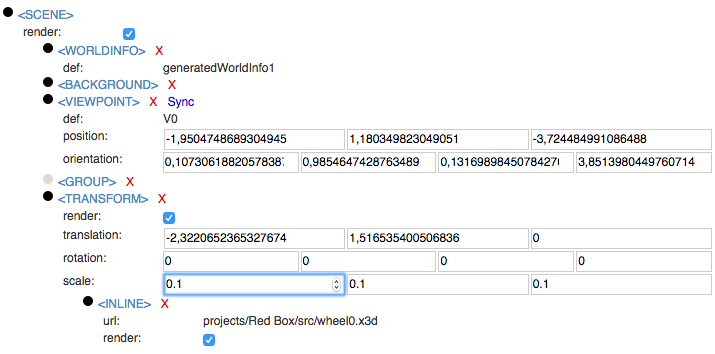
\includegraphics[width=\textwidth]{../assets/treeview.png}
  \caption{The rendered tree-view.}
  \label{fig:tree-view}
\end{figure}

\begin{figure}
  \centering
  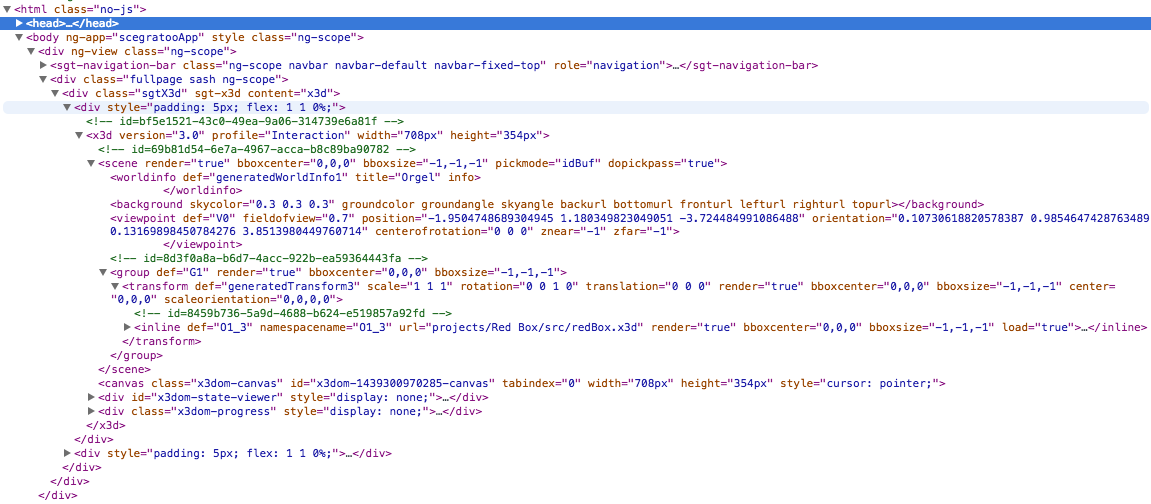
\includegraphics[width=\textwidth]{../assets/x3dom-dom.png}
  \caption{The \gls{X3D} scene inside the \gls{DOM}.}
  \label{fig:x3dom-dom}
\end{figure}

\begin{figure}
  \centering
  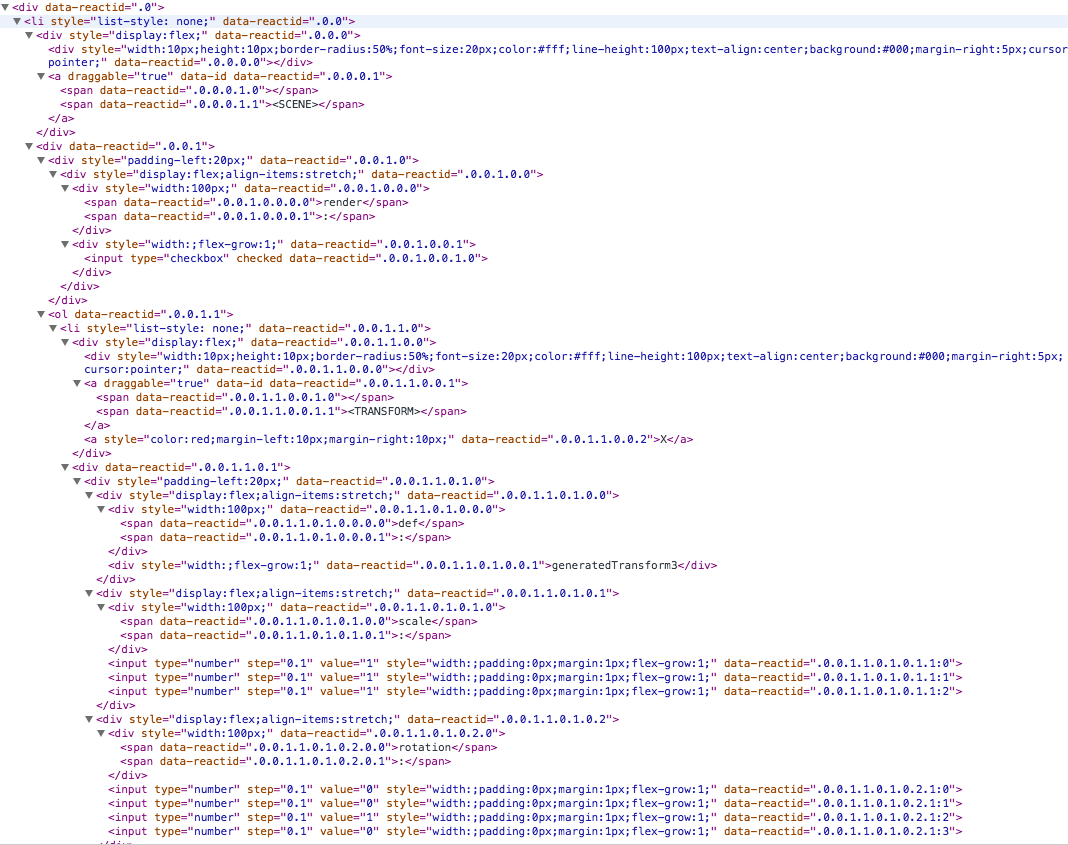
\includegraphics[width=\textwidth]{../assets/treeview-dom.png}
  \caption{About half of the \gls{DOM} elements that make up a tree-view of only three tree-view-nodes: a \texttt{scene}, \texttt{transform} and \texttt{inline} node.}
  \label{fig:treeview-dom}
\end{figure}

\begin{figure}
  \centering
  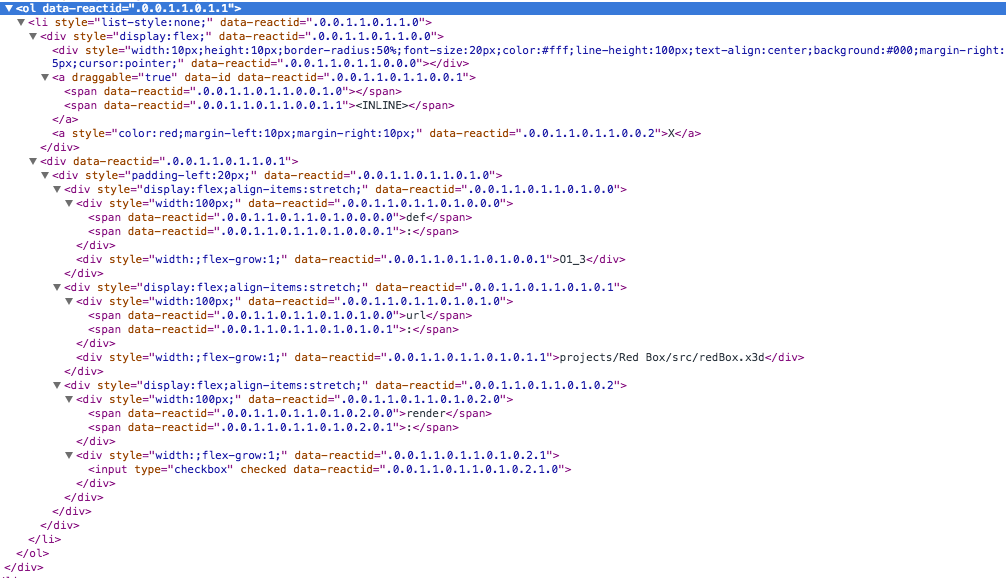
\includegraphics[width=\textwidth]{../assets/treeview-node-dom.png}
  \caption{The \gls{DOM} elements that make up a tree-view-node for an \texttt{inline}.}
  \label{fig:tree-view-node-dom}
\end{figure}

\begin{figure}
  \centering
  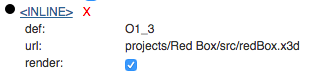
\includegraphics[width=.5\textwidth]{../assets/tree-view-node-rendered.png}
  \caption{The rendered tree-view-node of an \texttt{inline}.}
  \label{fig:tree-view-node-rendered}
\end{figure}

\begin{listing}
  \begin{minted}[breaklines,bgcolor=bg,linenos=true]{html}
<x3d version="3.0" profile="Interaction" width="708px" height="354px">
<!-- id=69b81d54-6e7a-4967-acca-b8c89ba90782 -->
<scene render="true" bboxcenter="0,0,0" bboxsize="-1,-1,-1" pickmode="idBuf" dopickpass="true">
<worldinfo>
</worldinfo>
<background skycolor="0.3 0.3 0.3"></background>
<viewpoint fieldofview="0.7" position="1 1 3" orientation="0.1 0.9 0.13 3.8">
</viewpoint>
<!-- id=8d3f0a8a-b6d7-4acc-922b-ea59364443fa -->
<group render="true" bboxcenter="0,0,0" bboxsize="-1,-1,-1">
  <transform render="true">
    <!-- id=8459b736-5a9d-4688-b624-e519857a92fd -->
    <inline url="projects/Red Box/src/redBox.x3d" render="true" load="true">
      <Shape render="true" isPickable="true">
        <Appearance sortType="auto" alphaClipThreshold="0.1">
          <Material diffuseColor="1 0 0" ambientIntensity="0.2" shininess="0.2"></Material>
        </Appearance>
        <Box solid="true" size="2,2,2"></Box>
      </Shape>
    </inline>
  </transform>
</group>
</scene>
</x3d>
  \end{minted}
	\caption{Generated \gls{X3D} example scene.}
	\label{list:x3dscene}
\end{listing}

\begin{listing}
  \begin{minted}[breaklines,bgcolor=bg,linenos=true]{html}
<div>
  <li>
    <div>
      <a> <span>SCENE</span> </a>
    </div>
    <div>
      <div>
        <div>
          <div>
            <span>render:</span>
          </div>
          <div>
            <input type="checkbox">
          </div>
        </div>
      </div>
      <ol>
        <li>
          <div>
            <a> <span>WORLDINFO</span> </a>
            <a>X</a>
          </div>
          <div>
            <div>
              <div>
                <div>
                  <span>def:</span>
                </div>
                <div>generatedWorldInfo1</div>
              </div>
            </div>
          </div>
...
      </ol>
    </div>
  </li>
</div>
  \end{minted}
  \caption{Simplified tree-view structure.}
  \label{list:tree-view}
\end{listing}

The aim is to keep the tree-view a consistent representation of the scene-graph.
The tree-view filters some nodes and attributes. As an example, nodes contained
in an \texttt{inline} are not shown, since  SceGraToo's task is only to compose
a scene of \texttt{inlines}, not to change something inside the \texttt{inlines}.
Also not all attributes are shown, but only the ones the user may be interested
in (such as \texttt{DEF}, \texttt{translate} or \texttt{rotate}).

One approach is to instantiate the tree-view-component with a
scene-graph-node as root node. For all child nodes, the tree-view-component
instatiates new tree-view-node-components. These tree-view-node-components
create the corresponding tree-view-nodes, while further traversing the
scene-graph. For each scene-graph-node a corresponding tree-view-node-component
is created. If there are no child nodes left, the tree-view creation is done.
Each tree-view-node-component creates all \gls{DOM} elements necessary to represent
the corresponding scene-graph-node in the \gls{DOM}. Also each
tree-view-node-component observes its corresponding scene-graph-node for
attribute mutations and added or removed child nodes and acts accordingly.

Depending on how the scene-graph is mutated, three main cases can be differentiated:

\begin{description*}
  \item[a scene-graph-node is added]
    A new tree-view-node-component is instantiated, adding all \gls{DOM} elements making up the tree-view-node to the \gls{DOM}.
  \item[a scene-graph-node is deleted]
    The corresponding tree-view-node-compo\-nent is destroyed and all \gls{DOM} elements making up that tree-view-node are removed from the \gls{DOM}.
  \item[a scene-graph-node is mutated]
    The corresponding \gls{DOM} elements that make up the  tree-view-node are altered to reflect the mutation.
\end{description*}

Tree-view-nodes can also be used to edit scene-graph nodes' properties. When an
input element, that contains the x value of a transformation, is edited, its
tree-view-node-component is notified of the change, by firing a change event, to
which the component subscribed, and applies the new value to the corresponding
scene-graph-node.

It is assumed, that the updates will always lead to a consistent state, where the
scene-graph and the tree node converge. It is also assumed, that an application
may be buggy and in that case the synchronization process has no ability to
detect if updates lead to an inconsistent state. It also has no ability to
recover from an inconsistent state.

In the following, two main issues are described.

\begin{description*}
  \item[Problem 1: keeping the tree-view consistent with the scene-graph]
    The difficulty, to make sure that incremental updates are error-free,
    exacerbates even more when further functionality is
    added to the tree-view,  like checkboxes for
    specific properties or saving state in the tree-view that is not part of
    the scene-graph, e.g~the possibility to collapse parts of the tree.
  \item[Problem 2: implementation effort]
    For every new feature four pieces of code have to be written:
    \begin{enumerate*}
      \item Source code for parsing the scene-graph
      \item Source code to generate the tree-view-node
      \item Source code to synchronize changes to a scene-graph-node to the corresponding tree-view-node
      \item Source code to synchronize changes to a tree-view-node to the corresponding scene-graph-node
    \end{enumerate*}
\end{description*}

This can be simplified if only the functionality for parsing the
scene-graph, and  for creating the \gls{DOM} elements that represent the scene-graph,
is implemented and, on every change, the whole tree-view is recreated by repeating these steps.

Problem 1 is solved completely, because incremental updates are gone and
Problem 2 is reduced to the following two steps:

\begin{enumerate*}
  \item Source code for parsing the scene-graph and generating the tree-view
  \item Source code to synchronize changes to a tree-view-node to the corresponding scene-graph-node
\end{enumerate*}

Rerendering the whole part of the \gls{DOM} on every change usually is inefficient. Removing a big part
of the \gls{DOM} and replacing it would lead to a \emph{reflow}, which is the browser's
process of laying out the content. This process is blocking, meaning the user can't
scroll or otherwise interact with the application. \cite{reflow}

React is used to minimize the possibility of a reflow. React
calculates a lightweight representation of what the \gls{DOM} (called the virtual DOM) should be like and
compares that to the present \gls{DOM}. It calculates a set of patches and
only applies these to the \gls{DOM}.

From a developer's point of view, the application is programmed like it is
completlely rerendered everytime something changes. From the browser's point
of view only a minimal set of changes, only those that are required to transform the
\gls{DOM} into the desired state, are applied, thus enormously reducing the risk of a \emph{reflow}.

The code below (Listings \ref{oldvirtdom}, \ref{newvirtdom} and \ref{patch}) is
for explanitary purposes to describe how react works. It does not resemble
react's implementation in any way:

\begin{listing}[H]
  \begin{minted}[breaklines,bgcolor=bg,linenos=true]{html}
<ol data-reactid=".0">
  <li data-reactid=".0.0">scene
    <ol data-reactid=".0.0.0">
      <li data-reactid=".0.0.0.0">transform
        <ol data-reactid=".0.0.0.0.0">
          <li data-reactid=".0.0.0.0.0.0">inline</li>
        </ol>
      </li>
    </ol>
  </li>
</ol>
  \end{minted}
  \caption{Old Virtual DOM}
  \label{oldvirtdom}
\end{listing}

\begin{listing}[H]
  \begin{minted}[breaklines,bgcolor=bg,linenos=true]{html}
<ol data-reactid=".0">
  <li data-reactid=".0.0">scene
    <ol data-reactid=".0.0.0">
      <li data-reactid=".0.0.0.0">transform
        <ol data-reactid=".0.0.0.0.0">
          <li data-reactid=".0.0.0.0.0.0">inline</li>
        </ol>
      </li>
      <li>group</li>
    </ol>
  </li>
</ol>
  \end{minted}
  \caption{Virtual DOM with newly created \texttt{li} node.}
  \label{newvirtdom}
\end{listing}

\begin{listing}[H]
  \begin{minted}[breaklines,bgcolor=bg,linenos=true]{javascript}
var li = document.createElement('li')
li.innerText = 'group'
document.querySelector('[data-reactid=".0.0.0"]')
  .appendChild(li)
  \end{minted}
  \caption{Patch}
  \label{patch}
\end{listing}

That means, as long as the code to parse the scene-graph and to generate the
lightweight representation of the tree-view is correct, the tree-view will
represent the current state of the scene-graph.

\paragraph{Data Binding}
\label{data-binding}

Another approach is to utilize templates and data binding. Frameworks (like
angular) or web components implementations (like polymer)
support templates and two way data binding. Following only
angular directives are examined, but the same should be possible with web
components.

An angular directive consists of a template and some
JavaScript containing logic for creating the directive or reacting to
events.

For each node a directive is instantiated, which creates a template
rendering the node. Also for each child it creates a new instance of
itself.

\textbf{Example:}

The rendered structure is shown in Listing \ref{list:templatedata}. The
\texttt{treenode} (Listing \ref{list:angular1}) expands into the node name and a
\texttt{nodelist} (Listing \ref{list:angular2}), that then expands into a list
of tree-nodes for each child node (Listing \ref{list:angular3}), that further
expand again (Listing \ref{list:angular4}). This recursive expanding stops when a
\texttt{treenode} is childless.

\begin{listing}[H]
  \begin{minted}[breaklines,bgcolor=bg,linenos=true]{javascript}
node: {
  name: "scene",
  children: [
    {
      name: "viewpoint"
    },
    {
      name: "worldinfo"
    }
  ]
}
  \end{minted}
  \caption{Example input data.}
  \label{list:templatedata}
\end{listing}

\begin{listing}[H]
  \begin{minted}[breaklines,bgcolor=bg,linenos=true]{html}
<treenode node="node">
</treenode>
  \end{minted}
  \caption{The initial template, node is the node from the data in Listing~\ref{list:templatedata}.}
  \label{list:angular1}
\end{listing}

\begin{listing}[H]
  \begin{minted}[breaklines,bgcolor=bg,linenos=true]{html}
<treenode node="node">
  <span>{{node.name}}</span>
  <nodelist ng-repeat='node in children' children='children'>
  </nodelist>
</treenode>
  \end{minted}
  \caption{The template expands itself, putting the node's name into a span and adding a nodelist directive, that expands the node's children.}
  \label{list:angular2}
\end{listing}

\begin{listing}[H]
  \begin{minted}[breaklines,bgcolor=bg,linenos=true]{html}
<treenode node="node">
  <span>{{node.name}}</span>
  <nodelist ng-repeat='node in children' children='children'>
    <treenode node="children[0]">
    </treenode>
    <treenode node="children[1]">
    </treenode>
  </nodelist>
</treenode>
  \end{minted}
  \caption{The nodelist expands the children array and renders a treenode for every child.}
  \label{list:angular3}
\end{listing}

\begin{listing}[H]
  \begin{minted}[breaklines,bgcolor=bg,linenos=true]{html}
<treenode node="node">
  <span>{{node.name}}</span>
  <nodelist ng-repeat='node in children' children='children'>
    <treenode node="children[0]">
      <span>{{node.name}}</span>
    </treenode>
    <treenode node="children[1]">
      <span>{{node.name}}</span>
    </treenode>
  </nodelist>
</treenode>
  \end{minted}
  \caption{The treenode directive expands the nodes and renders their names, since there are no nodes left to render they stop.}
  \label{list:angular4}
\end{listing}

% TODO: reword



This is an minimal example to demonstrate how angular directives work from a programmer's point of view.
The scene-graph is traversed and, for each eligible child node, a new
\texttt{treenode} is created. The double braces are angular's syntax
to denote data-binding in templates. Data from the elements scope is
automatically inserted and kept up to date. Then, the data-binding would
ensure, that the tree-view and the model are kept in sync when the
\texttt{treenode}'s attributes are changed and the other way around.

\subsection{Communication}
\label{interaction}

The client communicates with the server via a small HTTP API returning \gls{JSON} encoded data.
Issuing a GET request to \texttt{/projects} returns all projects stored on the server.
Issuing a GET request to \texttt{/projects/unicorn} returns all data about unicorn project.
